\documentclass[pstricks,mathserif]{beamer}
\usetheme{Hannover}
\usefonttheme[onlymath]{serif}


\usepackage{graphicx}
%\usepackage[T1]{fontenc}
\usepackage[utf8]{inputenc}
\usepackage{amsmath, amssymb,amsthm}
\usepackage{comment}
%\usepackage{url} 
\usepackage{bm}
%\usepackage{esint}
\usepackage{multirow}
%\usepackage{thmtools, thm-restate}
\usepackage{mathtools}
%\usepackage{framed}
%\usepackage{float}
%\usepackage{subcaption}
\usepackage{epstopdf}%New addition
%\usepackage{cite}
%\usepackage{subcaption}
\usepackage{subfig}
\usepackage[percent]{overpic}
\usepackage[absolute,overlay]{textpos}


\definecolor{firstcolor}{HTML}{F5F5FF}
\definecolor{secondcolor}{HTML}{EBEBFF}
\definecolor{thirdcolor}{HTML}{E0E0FF}
% Recreate the commands for equations
%\renewcommand*{\equationautorefname}{equation}
%\def\equationautorefname~#1\null{%equation~(#1)\null

%Trying to get a pyramid
  
\usepackage{tikz}
\usetikzlibrary{intersections}  
\usetikzlibrary{hobby}
%\usepackage{multido}
%\SpecialCoor  
%\def\Pyramid#1{%
%    \begin{pspicture}(#1,-#1)
%    \multido{\i=1+1}{#1}{%
%        \pstriangle(!#1 2 div \i\space neg)(\i,\i)
%        \uput[90](!#1 2 div \i\space neg){\char\numexpr\i+64}}
%    \end{pspicture}}

%Commands

\newcommand\irregularcircle[2]{% radius, irregularity
  \pgfextra {\pgfmathsetmacro\len{(#1)+rand*(#2)}}
  +(0:\len pt)
  \foreach \a in {10,20,...,350}{
    \pgfextra {\pgfmathsetmacro\len{(#1)+rand*(#2)}}
    -- +(\a:\len pt)
  } -- cycle
}

\newcommand{\party}[2]{\frac{\partial{#1}}{\partial{#2}}}

\title{Jet evolution in a dense QCD medium}
\author{Linnéa Gräns Samuelsson}
\institute % (optional)
{
  Internship at CEA Saclay\\
  Supervisors: Edmond Iancu and Gregory Soyez
}
\begin{document}


\frame{\titlepage}


%\section{Structure}
\section{Intro}

\begin{frame}


\minipage{0.3\textwidth}
\endminipage\hfill
\minipage{0.7\textwidth}
\begin{itemize}
\item \emph{the medium: a quark gluon plasma created in a heavy ion collision}
\item \emph{the jet: a collimated spray of particles generated via successive branchings of a parton with high energy produced in the collision}
\end{itemize}
\endminipage\hfill


\vspace*{1cm}


Structure of presentation:

\begin{itemize}
\item Context
\item Physics
\item Stochastics
\item Numerics
\end{itemize}

\vspace*{1cm}

\end{frame}

\section{Context}

\begin{frame}

%\frametitle{\small \flushleft HIC's, QGP's and jets}
Heavy ion collisions, quark gluon plasma and jets,\\
what we observe:

\begin{center}
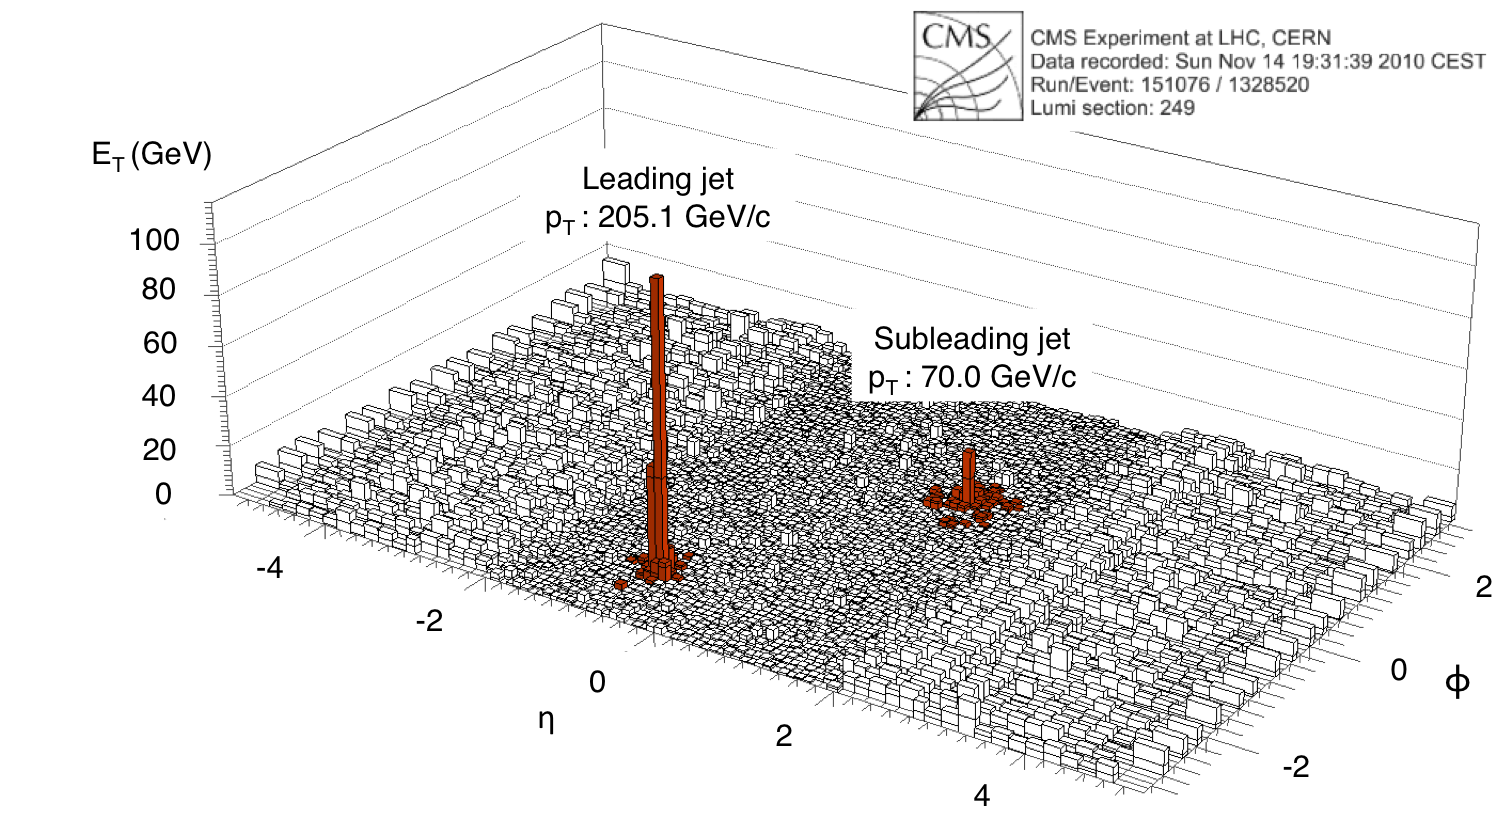
\includegraphics[width=1\linewidth]{CMS_JetQ.png}
\end{center}
%Note: this picture is misleading.
%This is one of the findings, fluctuations
%are large enough to compete with jets
%travelling a different distance through the medium

Di-jet asymmetry. Missing energy found among soft hadrons propagating at large angles $\Rightarrow$ different from in vacuum jet evolution.


\end{frame}



\begin{frame}
 %\begin{textblock}{0.5}(0.001,0.001)
 % Test
 %\end{textblock}
\vspace*{0.5cm}
Heavy ion collisions, quark gluon plasma and jets,\\
the stereotypical picture:
\begin{center}
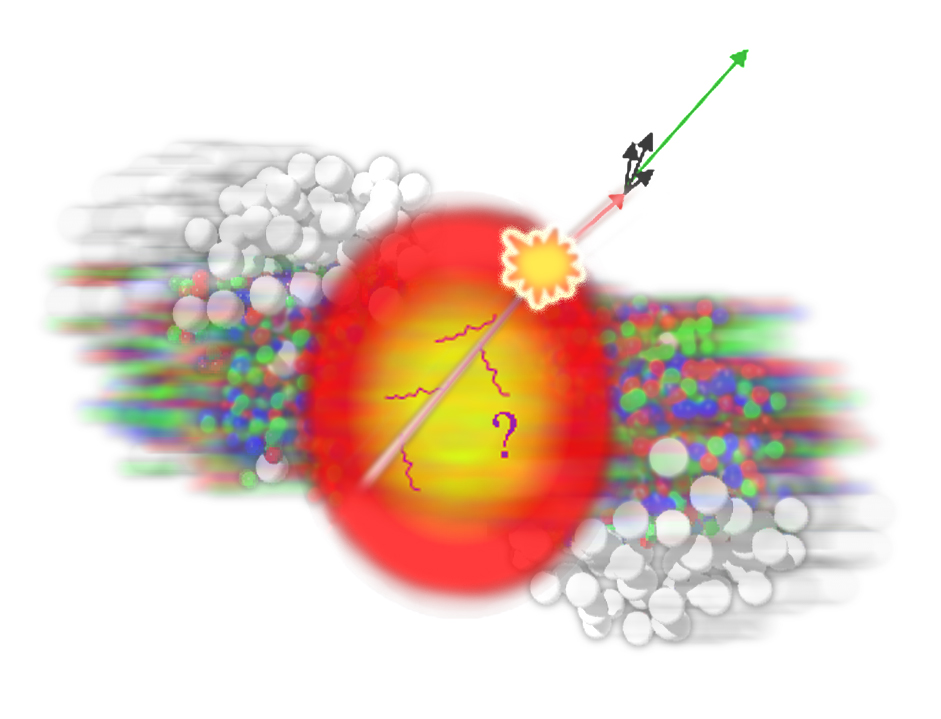
\includegraphics[width=0.45\linewidth]{jet-quenching.jpg}
\end{center}
%Note: this picture is misleading.
%This is one of the findings, fluctuations
%are large enough to compete with jets
%travelling a different distance through the medium


Implicit assumption: small energy fluctuations.

\vspace*{0.5cm}

\minipage{0.5\textwidth}
	\centering
	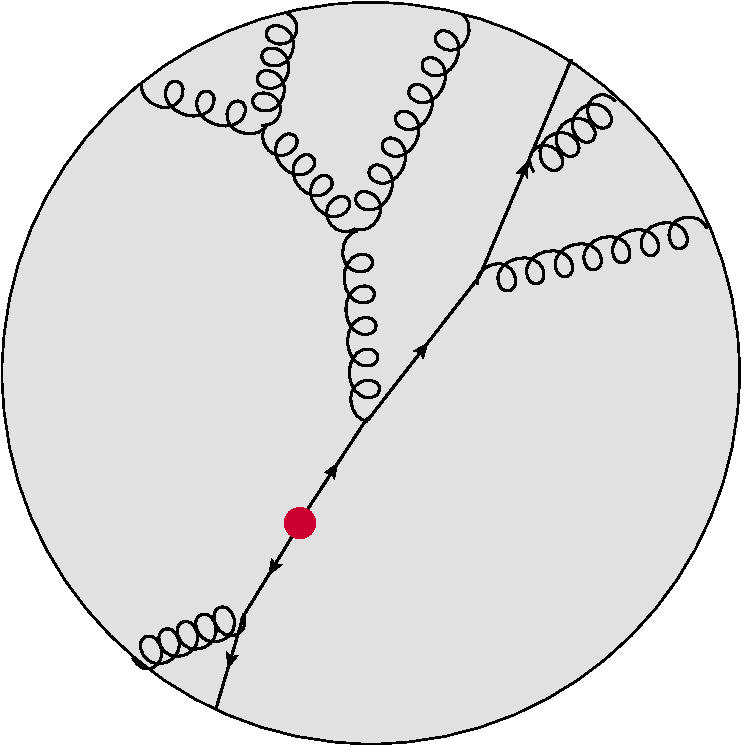
\includegraphics[width=0.45\linewidth]{Dijet_flucts1.pdf}
\endminipage\hfill
\minipage{0.5\textwidth}
	\centering
  	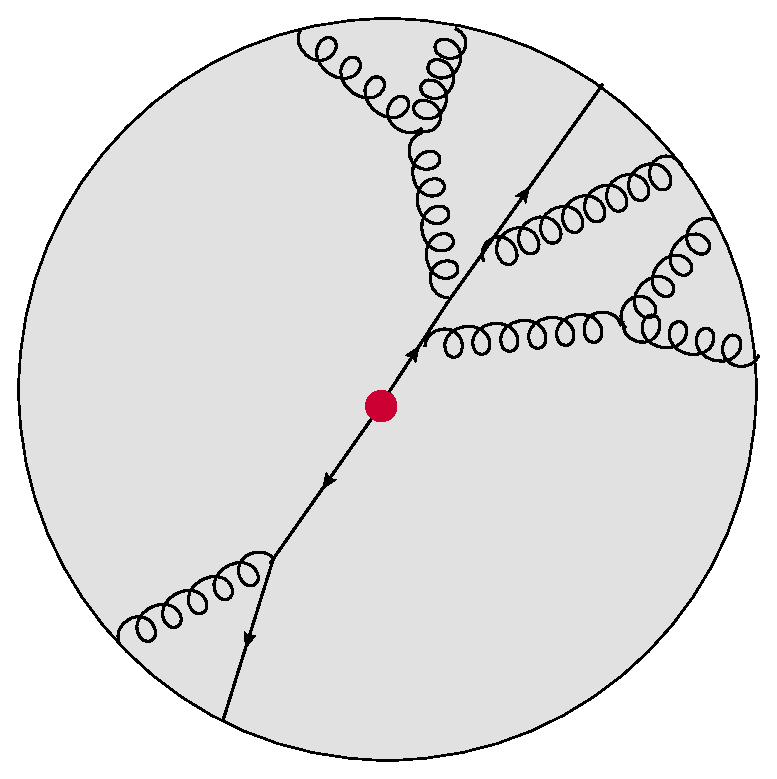
\includegraphics[width=0.45\linewidth]{Dijet_flucts2.eps}
\endminipage\hfill
\vspace*{1cm}

\end{frame}



\begin{frame}
We need a model that answers:
\begin{itemize}
\item How can the lost energy end up at such large angles?
\item How large are the energy fluctuations?
\end{itemize}
\end{frame}

\section{Physics}

\begin{frame}
\frametitle{Physics}
Start describing model, give expression for formation time and describe consequences of it, angles, multiple branching
\end{frame}

\begin{frame}
A typical event:

\begin{center}
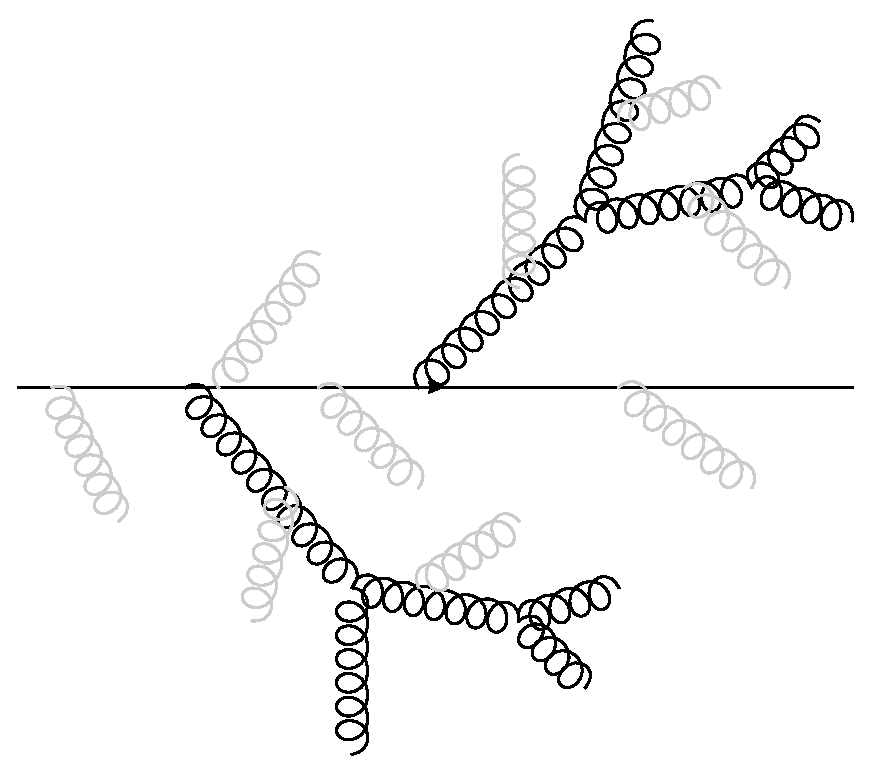
\includegraphics[width=0.5\linewidth]{democraticbranch.eps}
\end{center}

%
\begin{itemize}
\small
\item A number of $\mathcal{O}(1)$ of primary gluons emitted from leading particle.
\item They then branch democratically.
\item Grey gluon lines $=$ large number of non democratic, soft emissions.
\end{itemize}
%
%
\end{frame}


\section{Stochastics}



\begin{frame}
\frametitle{Stochastics}
In medium evolution as a Markovian process.


Describe D, D2, splitting kernels
\end{frame}



\begin{frame}

Energy fraction left in gluon cascade: $\int_0^1 \mathrm{d}x\, D(x,\tau) = e^{-\pi\tau^2}$\\ $\Rightarrow$ decreasing in time. Fate of lost energy, formally: condensate at $x=0$. Physically: thermalization.

\vspace*{1cm}
Note: (fix point...)
Democratic branching compared to wave turbulence:\\
~\\

{\tiny
\minipage{0.5\textwidth}
	\centering
	\begin{overpic}[width=0.7\linewidth]{democratic.eps}
	%\put(5,40){$x=1$}
	%\put(43,47){$x \sim \frac{1}{2}$}
	%\put(53,58){$x \sim \frac{1}{4}$}
	%\put(68,59){\vector(4,0){8}}
	%\put(64,70){$x \sim \frac{1}{8}$}
	%\put(79,71){\vector(4,0){8}}
	\end{overpic}
  	%\vspace*{-30pt}
  	%\caption{here go gluons}\label{fig:D0_t1}
\endminipage\hfill
\minipage{0.5\textwidth}
	\centering
  	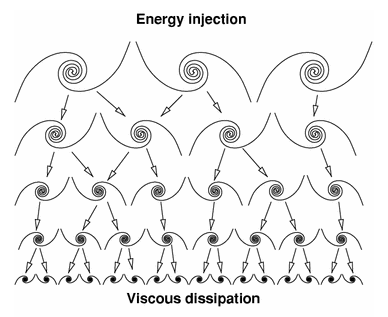
\includegraphics[width=0.7\linewidth]{Richardson_cascade.png}
  	%\vspace*{-30pt}
  	%\caption{Turbulence}\label{fig:D0_t5}
\endminipage\hfill
}


\end{frame}



\section{Numerics}

\begin{frame}
\frametitle{Numerics}
Numerical considerations, IR cutoff, pileup.

\begin{itemize}
\item $\epsilon$: IR cutoff for $x$ in splitting kernel
\item $x_{min}$: lowest $x$ considered
\end{itemize}


{
\centering
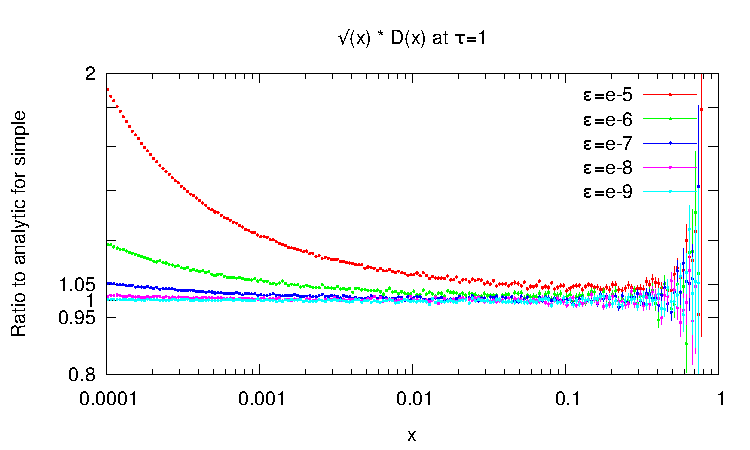
\includegraphics[width=1\linewidth]{convergence.pdf}
}

\end{frame}

\begin{frame}

Result: full kernel $\Rightarrow$ less efficient branching\\
~\\

%\vspace*{1cm}


\minipage{0.5\textwidth}
\centering
\small $\sqrt{x} D(x)$
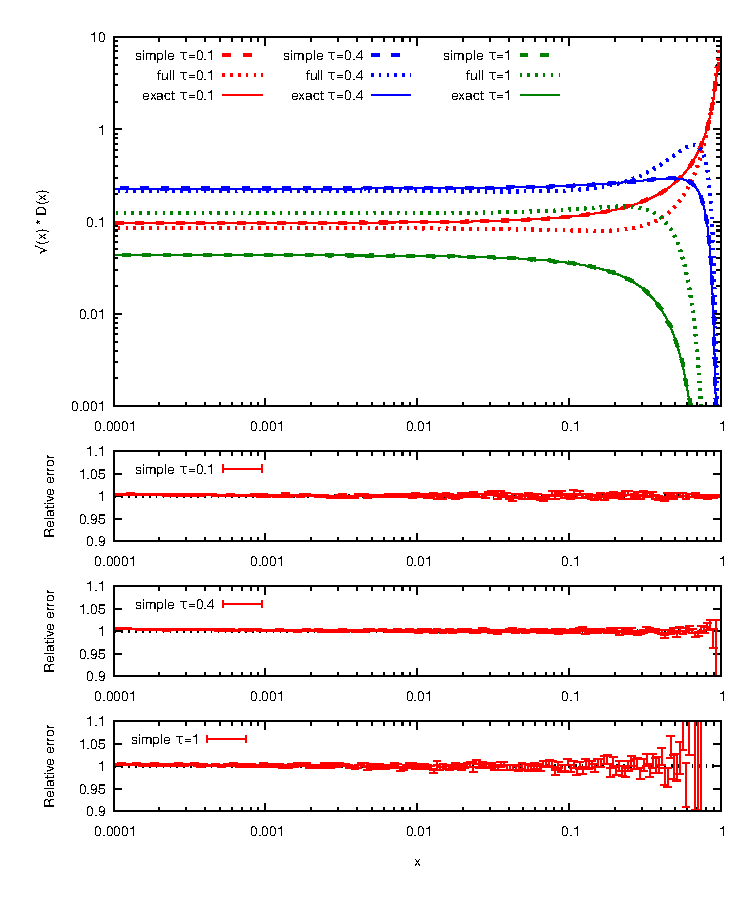
\includegraphics[width=1\linewidth]{times.pdf}
\endminipage\hfill
\minipage{0.5\textwidth}
%\centering
\small 

Simple splitting kernel, numerical versus analytic:
\begin{itemize}
\item Good agreement overall
\item Bias at small x (pileup)
\end{itemize}

Corrections from the full splitting kernel:
\begin{itemize}
\item Leading peak still present at $\tau=0.5$
\item Less energy lost at $\tau=1$
\end{itemize}
\endminipage\hfill


\end{frame}


\begin{frame}

Result: full kernel $\Rightarrow$ less efficient branching\\
~\\

%\vspace*{1cm}


\minipage{0.5\textwidth}
\centering
\small $\sqrt{x} D(x)$
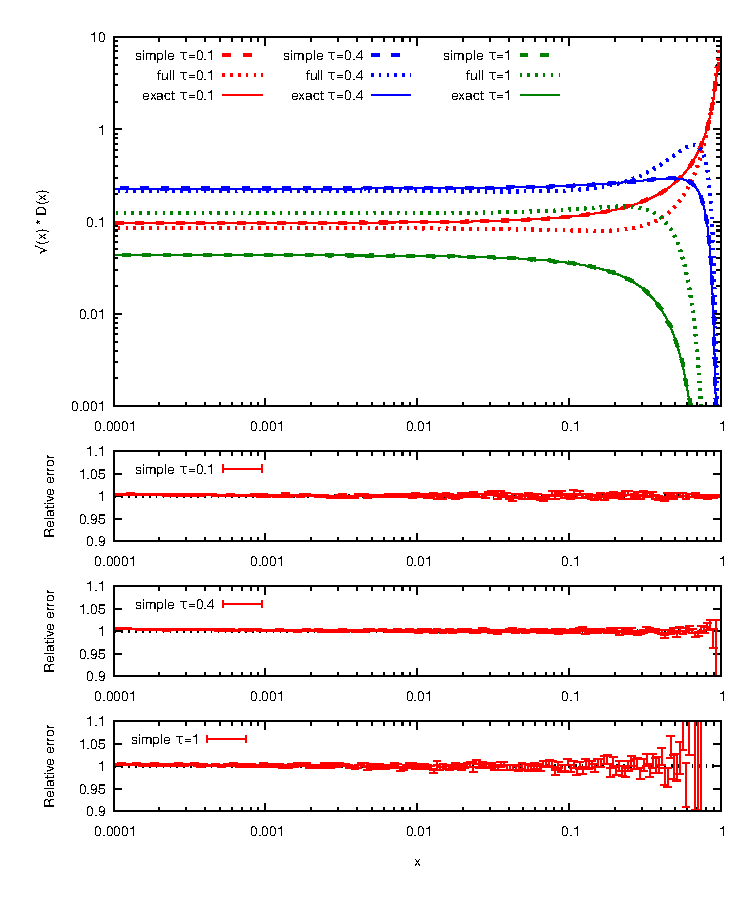
\includegraphics[width=1\linewidth]{times.pdf}
\endminipage\hfill
\minipage{0.5\textwidth}
\centering
\small $x D^2(x,x)$
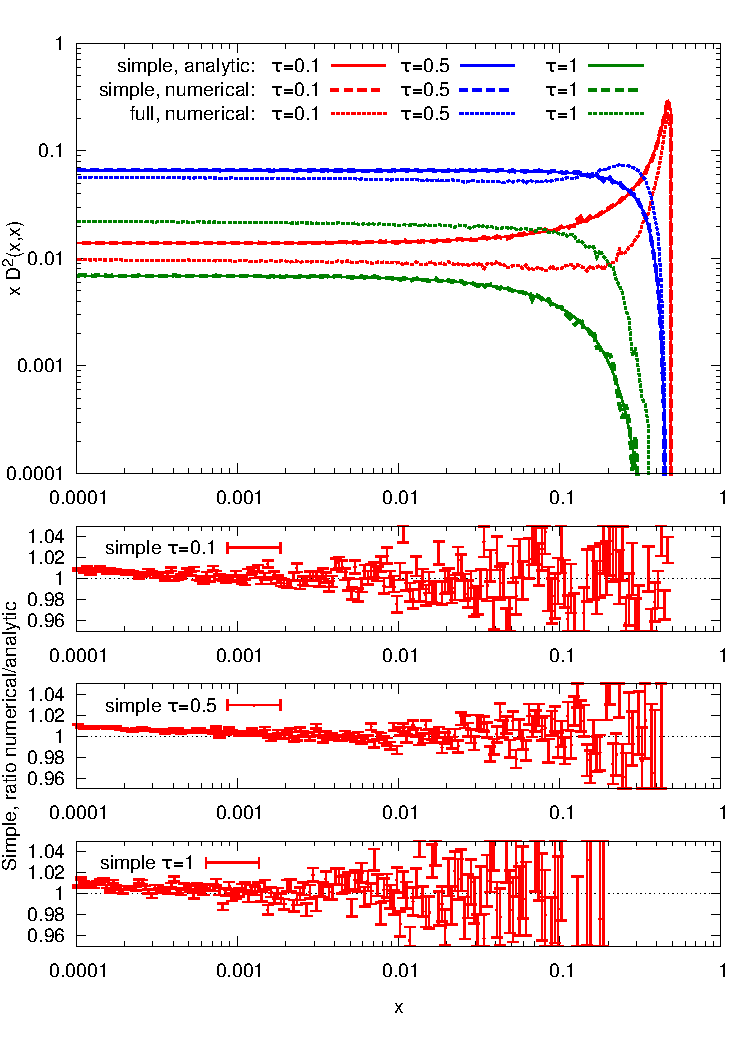
\includegraphics[width=1\linewidth]{D2.pdf}
\endminipage\hfill


\end{frame}



\begin{frame}
Energy loss: $1 - \int_0^1 \mathrm{d}x\, D(x,\tau) = 1 - e^{-\pi\tau^2}$
{\centering
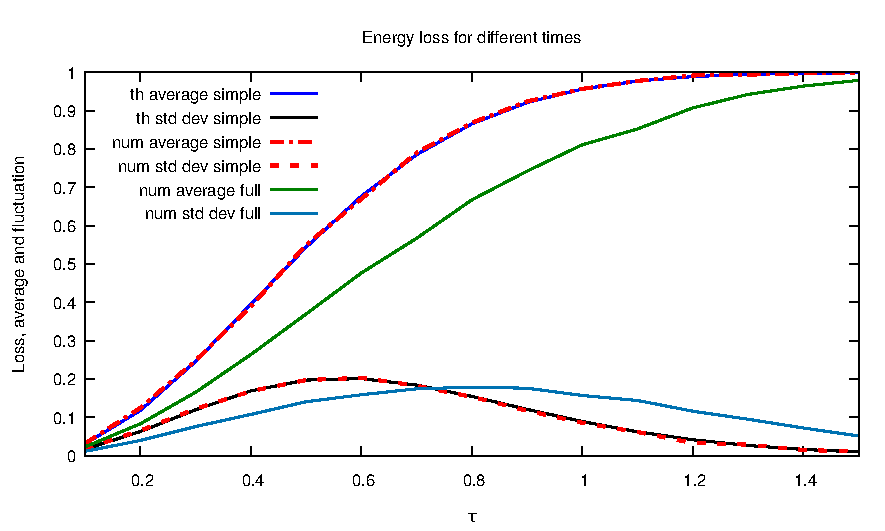
\includegraphics[width=1\linewidth]{energyloss.pdf}
}
\end{frame}



\section{Outro}
\begin{frame}

%Maybe something about future work, discussion etc. I should probably have the thesis itself in a pdf viewer for easy reference in case of questions.

Summary:

\begin{itemize}
\item Democratic branchings $\Rightarrow$ energy found at large angles
\item Prediction: large fluctuations in energy loss
\item Possible to make Monte Carlo simulation
\item Full kernel $\Rightarrow$ less efficient branching
\end{itemize}

Possible extensions:

\begin{itemize}
\item Things
\end{itemize}
~\\
\center THE END\\
~\\
Questions?

\end{frame}

\end{document}